\documentclass[11pt]{beamer}
\usetheme{CambridgeUS}
\usepackage[utf8]{inputenc}
\usepackage[french]{babel}
\usepackage[T1]{fontenc}
\usepackage{amsmath}
\usepackage{amsfonts}
\usepackage{amssymb}
\usepackage{graphicx}
\author{ O. Mory }
\title{Introduction à l'analyse des données}
%\setbeamercovered{transparent} 
%\setbeamertemplate{navigation symbols}{} 
%\logo{} 
\institute{LMI-SFA-UNA} 
%\date{} 
%\subject{} 
\begin{document}

\begin{frame}
\titlepage
\end{frame}

%\begin{frame}
%\tableofcontents
%\end{frame}

\begin{frame}{Les méthodes Usuelles}

\begin{itemize}
\item Analyse en Composantes Principales (A.C.P.) (K. Pearson, 1901)
\item Analyse factorielle des correspondances simples (A.F.C.)(Hirchsfeld, 1936)
\item Analyse factorielle des correspondances multiples (A.C.M.)(Guttman, 1941)
\item Méthodes de classification automatique
\end{itemize}

\end{frame}
\section{Analyse des données}
\begin{frame}{Analyse des données}

Analyser des données, c’est extraire d’une masse
d’informations brutes, des éléments de réponse aux
questions qui résultent des objectifs globaux
poursuivis.

\end{frame}

\begin{frame}{Analyse des données}

Traitement de données en masse 
\begin{itemize}
\item Grand nombre d’individus
\item Grand nombre de variables
\end{itemize}

\end{frame}

\begin{frame}{Analyse des données}
Développement parallèle à l’informatique

\begin{itemize}
\item Fichiers volumineux $\Rightarrow$ demande de méthodes
\item Capacité de calcul $\Rightarrow$ méthodes praticables
\end{itemize}
\end{frame}


\begin{frame}{Analyse des données}
Les outils mathématiques de l’analyse des données:

\begin{itemize}
\item Algèbre linéaire
\item Calcul matriciel
\end{itemize}
\end{frame}

\section{Méthodes factorielles}
\begin{frame}{Analyse des données}


Les outils mathématiques de l’analyse des données:

\begin{itemize}
\item Analyse en Composantes Principales (A.C.P.)

\item Analyse factorielle des correspondances\\
analyse de variables qualitatives
\begin{itemize}
\item Correspondances simples (A.F.C.) (Étude d’un
tableau de contingence)
\item Correspondances multiples (A.C.M.) (Utile lors du
dépouillement d’enquêtes)
\end{itemize}
\end{itemize}
\end{frame}


\begin{frame}{Introduction}

\begin{figure}
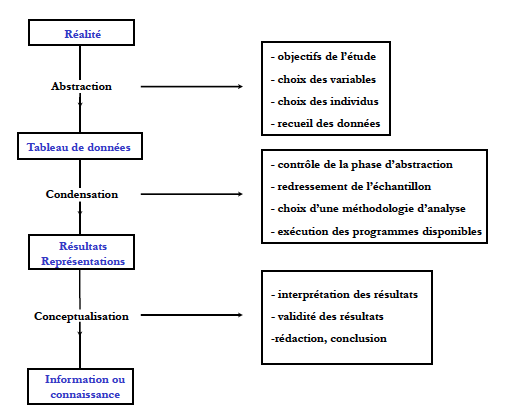
\includegraphics[scale=0.5]{schema2.png} 
\end{figure}
\end{frame}

\begin{frame}{Introduction}
\begin{figure}
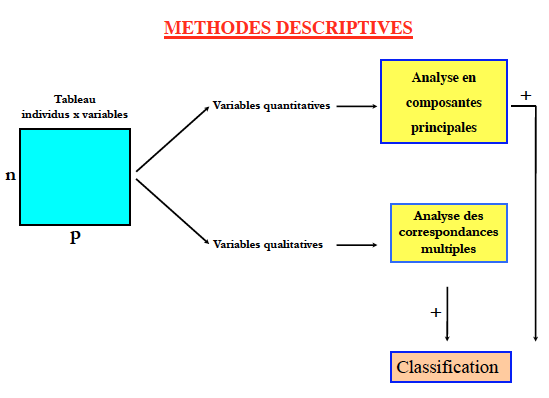
\includegraphics[scale=0.5]{schema1.png} 
\end{figure}
\end{frame}


\section{L’ANALYSE EN
COMPOSANTES PRINCIPALES
(A.C.P.)}

\begin{frame}{ACP}

Données : \\

$n$ individus observés sur $p$ variables quantitatives.
L’A.C.P. permet d’explorer les liaisons entre variables et les
ressemblances entre individus\\


Résultats\\

$\Rightarrow$ Visualisation des individus (Notion de distances entre individus)
 
$ \Rightarrow$ Visualisation des variables (en fonction de leurs corrélations)
\end{frame}

\begin{frame}{Interprétation des axes}

\begin{itemize}
\item Mesurer la qualité des représentations obtenues
\begin{itemize}
\item critère global
\item critères individuels
\end{itemize}
\item Utilisation éventuelle de variables supplémentaires
\end{itemize}
\end{frame}
\subsection{Formalisme du problème de ACP}
\begin{frame}{}

\begin{enumerate}
\item LES DONNÉES
\item PRINCIPE DE L’A.C.P.
\item LE CHOIX DE LA DISTANCE ENTRE INDIVIDUS
\item INERTIE TOTALE
\end{enumerate}

\end{frame}

\begin{frame}{Les données}
p variables quantitatives observées sur n individus.

\begin{figure}
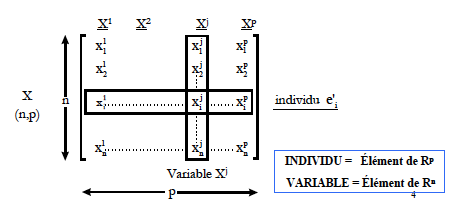
\includegraphics[scale=0.7]{schema3.png} 
\end{figure}

\end{frame}


\begin{frame}{On cherche à représenter le nuage des individus}

A chaque individu noté $e_i$, on peut associer un point dans
$R^p =$ espace des individus.\\

A chaque variable du tableau $X$ est associé un axe de $R^p$.

\begin{figure}
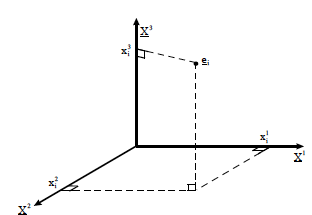
\includegraphics[scale=0.5]{schema4.png} 
\end{figure}
\centering
\begin{tabular}{|c|}
\hline 
\textcolor{blue}{{\Large Comment faire la représentation  4D?}}\\ 
\hline 
\end{tabular} 
\end{frame}

\subsection{Principe de l'ACP}
\begin{frame}{Principe de l'ACP}

\begin{block}{Principe}
On cherche une représentation des n individus , dans un
sous-espace $F_k$ de $R^p$ de dimension k<p ( k petit 2, 3 …; par exemple un plan)\\
Autrement dit, on cherche à définir $k$ nouvelles variables
combinaisons linéaires des $p$ variables initiales qui feront
perdre le moins d’information possible.
\end{block}



\begin{block}{Vocabulaire }
\begin{itemize}
\item Ces variables seront appelées «\textbf{composantes principales }»,
\item les axes qu’elles déterminent : « \textbf{axes principaux} »
\item les formes linéaires associées : « \textbf{facteurs principaux} »
\end{itemize}
\end{block}

\end{frame}


\begin{frame}
\begin{figure}
\includegraphics[scale=0.7]{schema5.png} 
\end{figure}

\textcolor{blue}{\textbf{{\Large Qu'espere t'on?}}}

\end{frame}

\begin{frame}
\begin{figure}
\includegraphics[scale=0.7]{schema5.png} 
\end{figure}

\textcolor{red}{\textbf{{\Large Qu'espere t'on?}}} $\Rightarrow$ \textcolor{blue}{\textbf{{\Large Perdre le moins d’information possible}}}  

\end{frame}


\begin{frame}

\begin{figure}
\includegraphics[scale=0.7]{schema6.png} 
\end{figure}

\end{frame}

\begin{frame}
\begin{figure}
\includegraphics[scale=0.7]{schema7.png} 
\end{figure}

\end{frame}

\subsection{LE CHOIX DE LA DISTANCE ENTRE INDIVIDUS}

\begin{frame}{Notion de distance euclidienne}

\begin{figure}
\includegraphics[scale=0.6]{schema8.png} 
\end{figure}

\textcolor{red}{{\Large \textbf{Que faire ?}  }}
\end{frame}


\begin{frame}{Normaliser}
Pour résoudre ce problème, on choisit de transformer les données en données centrées-réduites.\\
L’observation $x_i^k$ est alors remplacée par :

\begin{figure}
\includegraphics[scale=0.6]{schema9.png} 
\end{figure}

\end{frame}

\subsection{Inertie Totale}

\begin{frame}
\frametitle{Inertie}
\begin{figure}
\includegraphics[scale=0.6]{schema10.png} 
\end{figure}

\end{frame}

\begin{frame}
\frametitle{Inertie}
\begin{figure}
\includegraphics[scale=0.6]{schema11.png} 
\end{figure}

\end{frame}

\begin{frame}
\frametitle{Inertie}
\begin{figure}
\includegraphics[scale=0.6]{schema12.png} 
\end{figure}

\end{frame}
\begin{frame}
\frametitle{Inertie}
\begin{figure}
\includegraphics[scale=0.6]{schema13.png} 
\end{figure}

\end{frame}
\begin{frame}
\frametitle{Inertie}
\begin{figure}
\includegraphics[scale=0.6]{schema14.png} 
\end{figure}

\end{frame}

\section{Solution}
\begin{frame}
\frametitle{Axes principaux}
\begin{itemize}
\item On appelle axes principaux d’inertie les axes de direction
les vecteurs propres de V normés à 1.
\item Il y en a p.
\item Le premier axe est celui associé à la plus grande valeur
propre . On le note $u^1$
\item Le deuxième axe est celui associé à la deuxième valeur
propre . On le note $u^2$
\end{itemize}
\end{frame}


\begin{frame}
\frametitle{Composantes principales}
\begin{itemize}
\item À chaque axe est associée une variable appelée composante principale.
\item La composante c1 est le vecteur renfermant les cordonnées
des projections des individus sur l’axe 1.

\item La composante c2 est le vecteur renfermant les cordonnées
des projections des individus sur l’axe 2.


\item Pour obtenir ces coordonnées, on écrit que chaque
composante principale est une combinaison linéaire des
variables initiales.
\end{itemize}
$$ c^1=u_1^1*X^1+u_1^2*X^2+...+u_1^p*X^p$$
\end{frame}

\begin{frame}
\frametitle{PROPRIÉTÉS DES COMPOSANTES PRINCIPALES}
\begin{itemize}
\item La variance d’une composante principale est égale à
l’inertie portée par l’axe principal qui lui est associé.

\begin{itemize}

\item 1ère composante $c^1$ variance :
\item 2ème composante $c^2$ variance :
\item 3ème composante $c^3$ variance :

\end{itemize}
\item Les composantes principales sont non corrélées
deux à deux. En effet, les axes associés sont orthogonaux.
$\lambda_1$
\end{itemize}

\end{frame}

\begin{frame}{REPRÉSENTATION DES INDIVIDUS}

\begin{figure}
\includegraphics[scale=0.6]{schema15.png} 
\end{figure}

\end{frame}

\begin{frame}

\begin{figure}
\includegraphics[scale=0.6]{schema16.png} 
\end{figure}

\end{frame}


\begin{frame}{REPRÉSENTATION DES VARIABLES}

\begin{figure}
\includegraphics[scale=0.6]{schema17.png} 
\end{figure}

\end{frame}


\begin{frame}{INTERPRETATION DES « PROXIMITÉS » ENTRE
VARIABLES}

\begin{figure}
\includegraphics[scale=0.6]{schema18.png} 
\end{figure}

\end{frame}


\begin{frame}

\begin{figure}
\includegraphics[scale=0.6]{schema19.png} 
\end{figure}

\end{frame}


\begin{frame}{Coefficient de corrélation linéaire}

\begin{figure}
\includegraphics[scale=0.6]{schema20.png} 
\end{figure}

\end{frame}


\begin{frame}

\begin{figure}
\includegraphics[scale=0.6]{schema21.png} 
\end{figure}

\end{frame}


\begin{frame}{VALIDITÉ DES REPRÉSENTATIONS}

\begin{figure}
\includegraphics[scale=0.6]{schema22.png} 
\end{figure}

\end{frame}


\begin{frame}{Combien d’axes ?}

\begin{figure}
\includegraphics[scale=0.6]{schema23.png} 
\end{figure}

\end{frame}


\begin{frame}{}

\begin{figure}
\includegraphics[scale=0.6]{schema24.png} 
\end{figure}

\end{frame}


\begin{frame}{Contributions}

\begin{figure}
\includegraphics[scale=0.6]{schema25.png} 
\end{figure}

\end{frame}


\begin{frame}{REPRÉSENTATION DES VARIABLES}

\begin{figure}
\includegraphics[scale=0.6]{schema26.png} 
\end{figure}

\end{frame}


\end{document}